%\section{Multi-class Queuing Networks}
\section{Discrete-Event Dynamical System Model for Queuing Networks}
\label{section:model}



%\subsection{\label{subsec:deds}Discrete Event Dynamical System}

% We first begin with a general description of a \textbf{discrete event
% dynamical system} \textbf{(DEDS)}, which is specified by a tuple $(\mathcal{X},E,\mathcal{U},\phi,\phi',f)$.
% The system operates in continuous time $t\in\mathbb{R}_{+}$, and
% is defined by a state variable $x(t)\in\mathcal{X}$ and a finite
% set of events $E$ which update the state variable. For each event
% $e\in E$, there is an associated random variable $\tau^{e}\in\mathbb{R}_{+}$,
% drawn from a (possibly time-dependent) distribution $F_{e,t}$, which
% specifies the time remaining until the event occurs. We denote these
% as\textbf{ inter-event times}, and let $\tau^{E}\in\mathbb{R}_{+}^{|E|}$
% be the vector of inter-event times for all $e\in E$. 

% We consider a \textbf{controlled }discrete event dynamical systems,
% in which a controller takes an action $u\in\mathcal{U}$, which affects
% the dynamics through the event times. Specifically, the inter-event
% time $\tau^{e}$ of event $e$ is reshaped by the action into $\phi_{e}(\tau^{e},u)\in\mathbb{R}_{+}$.
% The next event that occurs is the event with the minimum reshaped
% inter-event time $e^{*}=\arg\min_{e\in E}\phi_{e}(\tau^{e},u)$ and
% we refer to this as the \textbf{focal event}. Once the event occurs,
% the state is updated, the event times for the non-focal events are
% decremented by the focal event time (potentially reshaped by the action
% as well $\phi'_{e}(\tau^{e^{*}},u)$), and the focal event time is
% reset by drawing a new event time $\tau^{e^{*}}\sim F_{e^{*}}$. The
% process repeats.

% Although the system evolves in continuous time, no changes to the
% state occur until an event happens. Thus, it is sufficient to sample
% the system only when event occurs. We index the sequence of events
% by $k\in\mathbb{N}$, so that $e_{1}$ is the first event to occur
% and $e_{k}$ is the $k$th event. We let $\tau_{k}$ be the $k$th
% inter-event epoch, i.e. the time elapsed between the $(k-1)$th and
% the $k$th time, and $t_{k}$ be the time of the $k$th event so that
% $t_{k}=\sum_{i=1}^{k}\tau_{j}$. We denote $\tau_{k}^{e}$ to be the
% residual inter-event time of event $e$ as soon as the $k$th event
% occurred, so that $\event_{k+1}=\arg\min_{e\in E}\phi_{e}(\tau_{k}^{e},u_{k})$
% and $\tau_{k+1}=\min_{e\in E}\phi_{e}(\tau_{k}^{e},u_{k})$. It is
% convenient to define $e(\tau_{k}^{E},u)=\arg\min_{e\in E}\phi_{e}(\tau_{k}^{e},u)$
% as the function mapping the inter-event times to the focal event.
% We let $u_{k}$ to denote the action taken at event time $t_{k}$,
% which influences the next event. This gives us the following transition
% function for $\tau_{k}$:

% \begin{align}
% \tau_{k+1} & =\min_{e\in E}\phi_{e}(\tau_{k}^{e},u_{k})\label{eq:time_transition}\\
% \tau_{k+1}^{e} & =\begin{cases}
% \tau_{k}^{e}-\phi'_{e}(\tau_{k+1},u_{k}) & \text{for }e\neq e_{k}\\
% \tau^{e}\sim F_{e,t_{k+1}} & \text{otherwise}
% \end{cases}
% \end{align}
% where $\tau^{e}\sim F_{e,t_{k+1}}$ is an event time randomly drawn
% from the distribution $F_{e,t}$ at $t=t_{k+1}$.

% The system is also defined by a \textbf{transition function} $f$,
% which specifies how the state evolves as function of the event that
% occurs. Starting from an initial state $x_{0}=x(0)$, we let $x_{k}:=x(t_{k})$
% be the state right after the $k$th event occurs. The dynamics of
% $x_{k}$ can be written as

% \[
% x_{k+1}=f(x_{k},\event_{k+1})
% \]

% \begin{defn}
% (Discrete Event Dynamical System) A discrete dynamical event system
% is a discrete time Markov Decision Process defined by a tuple $(\mathcal{X},E,\mathcal{U},\phi,\phi',f)$.
% Its augmented state $(x_{k},\tau_{k}^{E},t_{k})$ consists of the
% current state $x_{k}$, residual inter-event times $\tau_{k}^{E}$
% and the current time $t_{k}$. Starting from $(x_{0},\tau_{0}^{E},0)$,
% the augmented state $(x_{k},\tau_{k}^{E},t_{k})$ evolves as follows:

% \begin{align*}
% x_{k+1} & =f(x_{k},\event_{k+1})\tag{State Update}\\
% \event_{k+1} & =\arg\min_{e\in E}\phi_{e}(\tau_{k}^{e},u_{k})\tag{Event Selection}\\
% \tau_{k+1} & =\min_{e\in E}\phi_{e}(\tau_{k}^{e},u_{k})\tag{Inter-event Time}\\
% \text{\ensuremath{\tau_{k+1}^{e}}} & =\begin{cases}
% \tau_{k}^{e}-\phi'_{e}(\tau_{k},u_{k}) & \text{for }e\neq e_{k}\\
% \tau^{e}\sim F_{e,t_{k+1}} & \text{otherwise}
% \end{cases},\forall e\in E\tag{Inter-event Time Update}\\
% t_{k+1} & =t_{k}+\tau_{k+1}\tag{Time Update}
% \end{align*}
% This is a broad class of systems and has the capacity to represent
% any discrete-time Markov Decision Process.
% \end{defn}

% \begin{lem}
% Any discrete-time Markov Decision Process (MDP) with finite states
% and actions can be embedded as a discrete event dynamical system under
% exponential inter-event times $\tau^{e}\sim Exp(1)$.
% \end{lem}

% Given the wide generality of these systems, it is useful to discuss
% more structured discrete event dynamical systems. Of particular relevance
% for queuing networks are systems we denote as \textbf{linear discrete-event
% dynamical systems (Lin-DEDS)}. These systems involve linear updates
% to the state whenever an event occurs. For these systems, the state
% space is $\mathcal{X}\subseteq\mathbb{R}^{n}$ and events are represented
% as one-hot vectors, one for each of the $p=|E|$ events, i.e. $E=\{e^{i}:i\in[p]\}$
% where $e^{i}\in\{0,1\}^{p}$ is non-zero with $1$ in the $i$th component.
% The transition function is specified by two matrices $A\in\mathbb{R}^{n\times n}$
% and $D\in\mathbb{R}^{n\times p}$, so that it involves a linear
% function of the current state and event:

% \begin{equation}
% x_{k+1}=f(x_{k},\event_{k+1})=Ax_{k}+D \event_{k+1}\tag{Linear State Update}\label{eq:lin_state_equation}
% \end{equation}
% Given these dynamics, the interpretation of the $i$th column vector
% $D_{j}$ is as the shift contribution to the state update when
% the $i$th event occurs.
% \hntodo{Provide more detailed context on what our goal is. Why are we setting up all this notation? e.g., we're encoding the dynamics explicitly; deriving the exoMDP representation for queues. One way to achieve this is to move some of the discussion in S3 up here.}

% \hntodo{On a related note, one nice takeaway from this section is that you're writing the entire MDP in matrix vector notation, which essentially corresponds to the "pseudo-code". It'll be good to highlight this. }

% \hnlong{I recommend rethinking the current structure. Setting aside some of the high-level writing comments below, the main issue is that the reader will have to grind through Section 2 reading cumbersome matrix-vector description of a well-known system (for no perceivable reason). Then, we don't actually use any of this notation until Section 3.3. 

% For example, we can more clearly separate out the theoretical insights from the main methodology.  Since Section 3.2 can be stated anywhere in the paper (independent of Section 2), we can start with this "insight", then state the problem that the system is actually not differentiable so we cannot do IPA. Then in the next section, we can introduce the dynamics notation (current Section 2) AND its smoothed variant.

% Having said this, there may be many other structures that can work. Please think about the overall comment, not the specific suggestion.
% }

% \hnlong{You're writing an unusually good paper. Obviously I'm biased, but this work has the potential to become an instant classic. I'd like us to keep a long outlook on this work---it's conceivable that this paper will be read by graduate students 15 years later. We should keep this in mind when we write the paper. 

% Currently, we spend so much time discussing competing approaches before we introduce our framework. Perhaps we can reverse this and motivate and introduce our framework in a coherent way, then comparing to other approaches.

% As I detail in inline comments below, we should also highlight the ease of implementation and the engineering frameworks we rely on. We should emphasize that we are enabled by the autodifferentiation frameworks that allow us to compute pathwise gradients with virtually no effort. Even an explicit 2-line pseudo-code of straight-through (in PyTorch) would be good somewhere in the paper.
% Second, we need to highlight that literally every undergraduate in adjacent fields (including IEOR) knows how to use PyTorch these days. I believe our framework will be a democratizing force in solving queueing problems in that now anyone can view this as a SGD problem. 

% Obviously it's more complicated than this, but we should pitch this vision. This is what your conceptual framework is enabling!}

We describe multi-class queuing networks as discrete-event dynamical systems. This is different from the standard Markov chain representation, which is only applicable when inter-arrival and service times are exponentially distributed.
To accommodate more general event-time distributions, the system description not only involves the queue lengths, but also auxiliary information such as residual inter-arrival times and workloads. Surprisingly, this more detailed system description leads to a novel gradient estimation strategy (discussed in Section~\ref{section:gradient}) for policy optimization.

We first provide a brief overview of the basic scheduling problem. We then describe the discrete-event dynamics of multi-class queuing networks in detail and illustrate with a couple of well-known examples. While queuing networks have been treated as members of a more general class of Generalized Semi-Markov Processes (GSMPs) that reflect the discrete-event structure of these systems \cite{glynn1989gsmp}, we introduce a new set of notations tailored for queuing networks to elaborate on some of their special structures.
In particular, we represent the discrete event dynamics 
via matrix-vector notation that maps directly to its implementation in auto-differentiation frameworks, allowing for the differentiable simulation of large-scale queueing networks through GPU parallelization. 

\subsection{\label{subsec:control} The Scheduling Problem}

% \hntodo{This entire subsection should be given at the beginning of the section as overall context for what you're trying to do.}
A multi-class queuing network consists of $n$ queues and $m$ servers. The core state variable is the queue lengths associated with each queue, denoted as  $x(t) \in \N_{+}^{n}$, which evolves over continuous time. As a discrete-event dynamical system, the state also includes auxiliary data denoted as $\aux(t)$--- consisting of residual inter-arrival times and workloads at time $t$---which determines state transitions but are typically not visible to the controller.
% \hntodo{Most papers in queueing and applied probability reserve $o(t)$ for small-o notation. Perhaps change this?}

The goal of the controller is to route jobs to servers, represented by an assignment matrix $u \in \{0, 1 \}^{m \times n}$, to manage congestion. More concretely, the problem is to derive a policy $\pi(x)$, which only depends on the observed queue lengths and selects scheduling actions, to minimize the integral of some instantaneous costs $c(x,u)$. A typical instantaneous cost is a linear holding/waiting cost:
\[
c(x,u)=h^{\top}x
\]
% More concretely, the goal of the controller is to  $c(x,u,\xi)$
% be the instantaneous cost under state $x\in\mathcal{X}$ and action
% $u$ and sampled inter-event times.
% 
% lengths: e.g.
for some vector $h\in\R_{+}^{n}$. The objective is to find a
policy $\pi$ that minimizes the cumulative cost over a time horizon:
\begin{equation}
\min_{\pi}\mathbb{E}\left[\int_{0}^{T}c(x(t),\pi(x(t)))dt\right].\label{eq:time-average-cost}
\end{equation}
%a time-averaged cost over a fixed horizon $N$, measured in terms of the total number of events:
Optimizing a continuous time objective can be difficult and may require an expensive discretization procedure. However, discrete-event dynamical systems are more structured in that $x(t)$ is piecewise constant and is only updated when an {\bf event} occurs. For the multi-class queuing networks, events are either arrivals to the network or job completions, i.e., a server finishes processing a job.

It is then sufficient to sample the system only when an event occurs, and we can approximate the continuous-time objective with a performance objective in the discrete-event system over $N$ events,
\begin{equation}
\min_{\pi}
\left\{J_{N}(\pi) := \mathbb{E}\left[\sum_{k=0}^{N-1}c(x_{k},\pi(x_{k}))\tau_{k+1}^*\right]
\right\}
\label{eq:des-cost}
\end{equation}
where $x_k$ is the queue lengths after the $k$th event update. $\tau^{*}_{k+1}$ is an inter-event time that measures the time between the $k$th and $(k+1)$th event, and $N$ is chosen such that the time of the $N$th event, a random variable denoted as $t_{N}$, is ``close" to $T$.
%For this objective to well-approximate the continuous time counterpart, one would need to select $N$ large enough to so that the time of the $N$th event, a random variable denoted as $t_{N}$, is close to $T$.
% We multiply the cost after event $k$ by the inter-event epoch $\tau_{k+1}$
% %in order to properly average the cost by the duration. As a result, this will be 
% so that \eqref{eq:des-cost} is equivalent to the following continuous time objective for $T=t_{N}^*$,

The dynamics of queuing networks are highly stochastic, with large variations across trajectories. Randomness in the system is driven by the random arrival times of jobs and the random workloads (service requirements) of these jobs.  We let $\xi_{1:N}=\{\xi_{i}\}_{i=1}^{N}$ denote a single realization, or `trace', of these random variables over the horizon of $N$ events.
% Due to the exogenous structure of the discrete event system, we can % compute the cost of a policy under a single trace $\xi_{1:N}=\{\xi_{i}\}_{i=1}^{N}$;
We can then view the expected cost~\eqref{eq:des-cost} more explicitly as a policy cost averaged over traces. 
In addition, we focus on a parameterized family of policies $\{\pi_{\theta}:\theta\in\Theta\}$, for some $\Theta\subseteq\R^{d}$, in order to optimize~\eqref{eq:des-cost} efficiently. In this case, we utilize the following shorthand $J_N(\theta;\xi_{1:N})$ for the
policy cost over a single trace and $J_N(\theta)$ for the average policy
cost under $\pi_{\theta}$,
which leads to the parameterized control problem:
\begin{equation}
\min_{\theta}
\left\{J_{N}(\theta) := \mathbb{E}\left[J(\theta;\xi_{1:N})\right]
:= 
\mathbb{E}\left[\sum_{k=0}^{N-1}c(x_{k},\pi_{\theta}(x_{k}))\tau^{*}_{k+1}\right]
\right\}.
\label{eq:param-cost}
\end{equation}
We now turn to describe the structure of the transition dynamics of multi-class queuing networks, to elaborate how scheduling actions affect the queue lengths.

% Under exponentially distributed inter-arrival and service times, we
% can oftentimes represent the dynamics of the queuing network as a relatively simple discrete-time Markov chain (DTMC) via uniformization and proper truncation.\hntodo{CITE} To handle non-exponentially distributed system inputs, we also need to keep track of the residual inter-arrival and service times to have a Markovian system descriptor. On the other hand, discrete-event simulation is a standard modeling approach that can accommodate general system inputs. We find that its structure enables novel gradient estimation strategies (discussed in Section~\ref{section:gradient}) for policy optimization.

\subsection{System Description}
Recall that the multi-class queuing network consists of $n$ queues and $m$ servers, where each queue is associated with a job class, and different servers can be of different compatibilities with various job classes. Recall that $x(t)\in\mathbb{N}_{+}^{n}$ denotes the lengths of the queues at time $t \in \R_{+}$.
% A typical queuing network is composed of $n$ queues and $m$ servers, where each queue is associated with a job class. Let $x(t)\in\mathbb{N}_{+}^{n}$ denote the lengths of the queues at time $t$. It is updated by stochastic job arrivals and job departures when jobs are processed by the servers. The topology of the network is described by a matrix $M\in\{0,1\}^{m\times n}$ indicating which job class can be served by which server. In this work, we restrict ourselves to multi-class queuing networks where each job class has at most 1 compatible server.
% \begin{assumption}
% For every job class $j$, there is at most 1 compatible server $i$,
% i.e., $\sum_{i=1}^{m}M_{ij}\leq1$.
% \end{assumptions
%
% Let $x(t)\in\mathbb{N}_{+}^{n}$ denote the lengths of the queues at time $t$. 
% %The queue lengths are updated by stochastic job arrivals and job departures as jobs are processed by the servers. 
% The topology of the network is described by a matrix $M\in\{0,1\}^{m\times n}$ indicating which job class can be served by which server. In this work, we restrict ourselves to multi-class queuing networks where each job class has exactly 1 compatible server.
% \begin{assumption}
% For every job class $j$, there is 1 compatible server $i$,
% i.e., $\sum_{i=1}^{m}M_{ij}=1$.
% \end{assumption}
% We restrict our focus to this class of queues so that it is sufficient to track the service requirements of the top-of-the-queue jobs. Consequently, we do not need to make any assumptions about the order in which jobs within each queue are served (e.g., first-in-first-out (FIFO) or last-in-first-out (LIFO)), as long as the order is not state-dependent.
The queue lengths $x(t)$ are updated by one of two types of events: job arrivals or job completions. 
Although the process evolves in continuous time, it is sufficient to track the system only when an event occurs. We let $k\in \N_{+}$ count the $k$th event in the system, and let $t_{k}$ denote the time immediately after the $k$th event occurs. By doing so, we arrive at a discrete-time representation of the system. Given that we do not assume event times are exponential, the queue lengths $x_{k}$ alone are not a Markovian descriptor of the system. Instead, we must consider an  {\bf augmented state} $s_{k} = (x_{k}, \aux_{k})$, where $x_k \in \N^{n}_{+}$ is the vector of {\bf queue lengths} and $\aux_{k} = (\tau_{k}^{A}, w_{k}),\in \R^{2n}_{+}$ is an auxiliary state vector that includes {\bf residual inter-arrival times} $\tau_{k}^{A} = \{ \arrival \}_{j = 1}^{n} \in \R^{n}_{+}$ and {\bf residual workloads} $w_{k} = \{ \service \}_{j = 1}^{n} \in \R^{n}_{+}$ of the `top-of-queue' jobs in each queue. The auxiliary state variables determine the sequence of events.

More explicitly, for each queue $j\in[n]$, the residual inter-arrival time $\arrival$ keeps track of the time remaining until the next arrival to queue $j$ occurs. Immediately after an arrival to queue $j$ occurs, the next inter-arrival time is drawn from a probability distribution $F_{j}^{A}$. When a job arrives to queue $j$, it comes with a workload (service requirement) drawn from a distribution $F_{j}^{S}$. We allow the distributions $F_{j}^{A}$'s and $F_{j}^{S}$'s to vary with time, i.e., the interarrival times and service requirements can be time-varying. For notational simplicity, we will not explicitly denote the time dependence here. We refer to the residual workload at time $t_{k}$ of the top-of-queue job in queue $j$ as $\service$, which specifies how much work must be done before the job completion. A job is only processed if it is routed to a server $i\in[m]$, in which case the server processes the job at a constant service rate $\mu_{ij} \in \R_{+}$. We refer to $\mu \in \R_{+}^{m \times n}$  as the matrix of service rates.
Under this scheduling decision, the \textbf{residual processing time}, i.e., the amount of time required
to process the job, is $\tau^{S}_{k,j}= \service/\mu_{ij}$. 
% We emphasize that it is the processing time \emph{not} the raw workload $\service$ that determines when the job is processed, and this is directly influenced by the actions taken by the controller.
% We
% denote $\mu\in\mathbb{R}_{+}^{m\times n}$ as the matrix of service rates where $\mu_{ij}$ is the service rate for server $i$ serving job class $j$.

% Although the process evolves in continuous time, it is sufficient to track the system only when an event occurs. Doing so, we arrive at a discrete-time representation of the system: $s_{k} = (x_{k}, \tau_{k})$, where $x_k \in \N^{n}_{+}$ is the vector queue lengths and $\tau_{k} \in \R^{2n}_{+}$ is the vector of {\bf residual event times } (i.e., interarrival and service times) immediately after the $k$th event occurs. Unlike the Markovian representation of queuing networks under exponential event times, our description is more general and includes the residual event times as state variables, even though typical queuing policies do not explicitly use this information.

The augmented state $s_{k}$ is a valid Markovian descriptor of the system and we now describe the corresponding  transition function $f$ such that
\[
s_{k+1} = f(s_{k}, u_{k}, \xi_{k+1}),
\]
where $u_{k}$ is an action taken by the controller and $\xi_{k+1}$ contains external randomness arising from new inter-arrival times or workloads drawn from $F^{A}_{j}$'s or $F^{S}_{j}$'s depending on the event type.

The transition is based on the next event, which is the event with the minimum residual time. The controller influences the transitions through the processing times, by deciding which jobs get routed to which servers. We focus on scheduling problems where the space of controls $\mathcal{U}$ are feasible assignments of servers to queues. Let $\ones_{n}\in \R^{n}$ denote an $n$-dimensional vector consisting of all ones. The action space is, 
\begin{equation}
\label{eq:action_space}
\mathcal{U}:=\left\{ u\in\{0,1\}^{m\times n}:u\ones_{n} = \ones_{m}, \ones_{m}^{\top} u=\ones_{n},u\leq M\right\},
\end{equation}
where $M\in\{0,1\}^{m\times n}$ is the {\bf topology} of the network, which indicates which job class can be served by which server. Following existing works on scheduling in queuing networks~\cite{meyn2008control}, we consider networks for which each job class has exactly 1 compatible server.
\begin{assumption} \label{ass:queue}
%(Scheduling) 
For every queue $j$, there is 1 compatible server,
i.e., $\sum_{i=1}^{m}M_{ij}=1$.
\end{assumption}
% We restrict our focus to this class of queues so that it is sufficient to track the service requirements of the top-of-the-queue jobs. Consequently, we do not need to make any assumptions about the order in which jobs within each queue are served (e.g., first-in-first-out (FIFO) or last-in-first-out (LIFO)), as long as the order is not state-dependent.

\begin{figure}[t]
\hspace{-1em}
    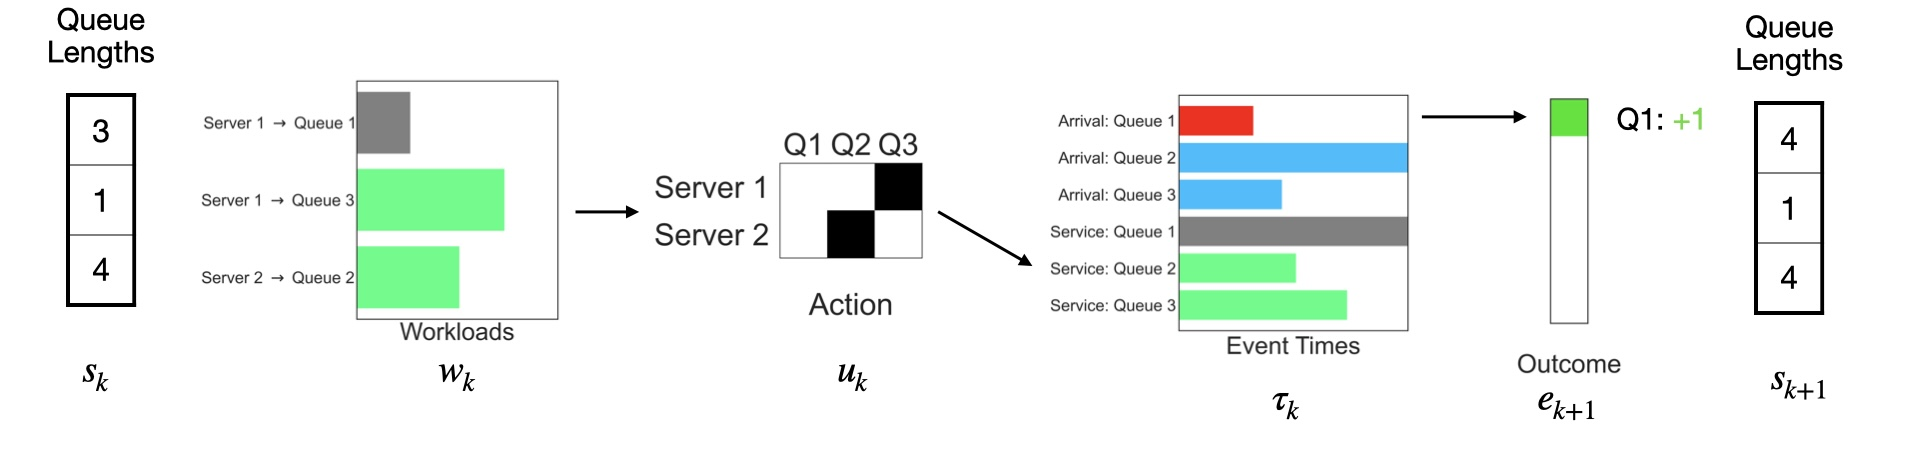
\includegraphics[height = 1.7in]{plot/gradient/one_step.jpeg}
    
    \caption{One step of the dynamics for the criss-cross network (see Example~\ref{example:criss-cross} and Figure~\ref{fig:networks}). There are 3 queues and 2 servers. Beginning with queue-lengths $x_{k} = (3, 1, 4)$ and workloads $w_{k}$, the action $u_{k}$ assigns server 1 to queue 3 and server 2 to queue 2. The workloads of the selected queues are highlighted in light green. As a result, the valid events are arrivals to queue 1 and queue 3 (queue 2 has no external arrivals) and job completions for queue 2 and queue 3 (queue 1 cannot experience any job completions because no server is assigned). The arrival event to queue 1 has the minimum residual time (highlighted in red) so it is the next event, and $e_{k+1}$ is a one-hot vector indicating this. Since an arrival occurred, the  queue-lengths are updated as $x_{k+1} = (4, 1, 4)$.}
    \label{fig:one_step}
\end{figure}

Given an action $u$, the residual processing time is $\service/\mu_{ij}$ when $u_{ij}=1$ and $\infty$ 
when $u_{ij}=0$. This can be written compactly as 
% \begin{align*}
% \phi_{A_{j}}(\tau^{A_{j}},u) & =\tau_{k,i}^{A}\\
% \phi_{S_{j}}(\tau^{S_{j}},u) & =\frac{\service}{u_{j}^{\top}\mu_{j}}:=\frac{\service}{\sum_{j=1}^{m}u_{ij}\mu_{ij}}
% \end{align*}
\begin{equation}
\label{eqn:processing_time}
\tau^{S}_{k,j} \equiv \frac{\service}{\sum_{i=1}^{m}u_{ij}\mu_{ij}} = \frac{\service}{\servicemap_{j,j}},
\end{equation}
where $\mathbf{diag}(u^{\top} \mu) \in \R^{n \times n}$ extracts the diagonal entries of the matrix $u^{\top} \mu \in \R^{n \times n}$.

As a result, at time $t_{k}$ the {\bf residual event times} $\tau_{k} \in \R_{+}^{2n}$ consists of the residual inter-arrival and processing times,
% We let $\servicemap_{u} \in \R^{2n \times 2n}_{+}$ be a (diagonal) matrix that converts the residual service requirements $\tau_{k}$ to the residual processing times (while keeping the inter-arrival times the same),
% \[
% V_{u_{k}}\tau_{k} = \left(
% \tau_{k}^{A_{1}},...,\tau_{k}^{A_{n}},
% (u_{1}^{\top}\mu_{1})^{-1} \tau_{k}^{S_{1}},...,(u_{n}^{\top}\mu_{n})^{-1} \tau_{k}^{S_{n}}
% \right) \in \R^{2n}_{+}
% \]
\[
\tau_{k} \equiv (\tau_{k}^{A}, \tau_{k}^{S}) = (\tau_{k}^{A}, \servicemapk^{-1} \servicek )
\]
We emphasize that $\tau_{k}$ depends on the action $u$. The core operation in the transition dynamics is the {\bf event selection} mechanism. The next event is the one with the minimum residual time in $\tau_{k}$.
%(arrival time or processing time). 
We define $\event_{k+1} \in \{0,1\}^{2n}$ to be a one-hot vector representing the $\argmin$ of $\tau_{k}$ -- the position of the minimum in $\tau_{k}$:
\begin{align*}
\event_{k+1}(\aux_{k}, u_{k}) &\equiv \argmin (\tau_{k})  \in \{0,1\}^{2n}\tag{Event Select}
%& = \argmin \{ \tau_{k}^{A} , \servicemapk^{-1} \servicek \} 
%\in \{0,1\}^{2n}
\end{align*}
$\event_{k+1}(\aux_{k}, u_{k})$ indicates the type of the $(k+1)$th event.
In particular, if the minimum residual event time is a residual inter-arrival time, then the next event is an arrival to the system. If it is a residual job processing time, then the next event is a job completion.
We denote $\tau^{*}_{k+1}$ to be the {\bf inter-event time}, which is equal to the minimum residual time:
\begin{align}
\tau^{*}_{k+1}(\aux_{k}, u_{k}) 
= \min \{ \tau_{k} \}
\tag{Event Time}
\end{align}
$\tau^{*}_{k+1}(\aux_{k}, u_{k})$ is the time between the $k$th and $(k+1)$th event, i.e. $t_{k+1} - t_{k}$.

After the job is processed by a server, it either leaves the system or proceeds
to another queue. Let $R\in\mathbb{R}^{n\times n}$ denote the {\bf routing matrix}, where the jth column, $R_{j}$ details the change in the queue lengths when a job in class $j$ finishes service. For example, for a tandem queue with two queues, the routing
matrix is
\[
R=\left[\begin{array}{cc}
-1 & 0\\
1 & -1
\end{array}\right]
\]
indicating that when a job in the first queue completes service, it leaves its
own queue and joins the second queue. When a job in the second queue
completes service, it leaves the system. 
%We can incorporate probabilistic routing through random routing matrices.
%We can then write the update to the queue-lengths as involving 

We define the {\bf event matrix} $D$ as a  block matrix of the form
\[
D=[\begin{array}{cc}
I_{n} & R\end{array}],
\]
where $I_n$ is the $n\times n$ identity matrix. The event matrix determines the update to the queue lengths, depending on which event took place. In particular, when the $(k+1)$th event occurs, the update to the queue lengths is
\begin{align}
x_{k+1} &=x_{k}+D \event_{k+1}(\aux_{k}, u_{k})
\tag{Queue Update} 
\end{align}
Intuitively, the queue length of queue $j$ increases by $1$ when the next event is a class $j$ job arrival; the queue lengths update according to $R_{j}$ when the next event is a queue $j$ job completion.

The updates to the auxiliary state $\aux_{k} = (\tau_{k}^{A}, w_{k}) \in \R_{+}^{2n}$ is typically given by
% \begin{align}
% \tau_{k+1}^{A} &= \tau_{k}^{A} - \tau_{k+1}^{*}\ones_{n} + T e_{k+1},
% \quad T_{j} \stackrel{iid}{\sim} F_{j}^{A} \\
% w_{k+1} &= \servicek - \tau_{k+1}^{*} \mathbf{diag}(u^\top \mu) + We_{k+1},
% \quad W_{j} \stackrel{iid}{\sim} F_{j}^{A}
% \end{align}
\begin{align}\label{eq:aux_update}
\left[
\begin{array}{c}
\tau_{k+1}^{A} \\
w_{k+1}
\end{array}
\right]
&= 
\left[
\begin{array}{c}
\tau_{k}^{A} \\
w_{k}
\end{array}
\right]
- 
\underbrace{\tau_{k+1}^{*}\left[
\begin{array}{c}
\ones_{n} \\
\servicemapk
\end{array}
\right]
}_{\text{reduce residual times}} + 
\underbrace{
\left[
\begin{array}{c}
T_{k+1} \\
W_{k+1}
\end{array}
\right] \odot e_{k+1}
}_{\text{draw new times / workloads}}
\hspace{-5em}
\tag{Aux Update} 
\end{align}
where $\odot$ is the element-wise product and
$T_{k+1} =\{T_{(k+1),j}\}_{j=1}^{n} \in \R^{n}$ are new inter-arrival times $T_{(k+1),j}  \sim F_{j}^{A}$ %if an arrival occurs. 
and $W_{k+1} = \{W_{k+1,j}\}_{j=1}^{n}\in \R^{n}$ are workloads $W_{k+1,j}  \sim F_{j}^{S}$.
%If the next event is a class $j$ job arrival occurs, we take a new inter-arrival time $T_{(k+1),j}$ from $T_{k+1}$ to update $\tau_{k+1}^A$. If the next event is a new queue $j$ job completion and queue $j$ is not empty, we take a new workload $W_{(k+1),j}$ from $W_{k+1}$ to update $w_{k+1,j}$. 
Intuitively, after an event occurs, we reduce the residual inter-arrival times by the inter-event time. We reduce workloads by the amount of work applied to the job, i.e., the inter-event time multiplied by the service rate of the allocated server. Finally, if an arrival occurred we draw a new inter-arrival time; if a job was completed, we draw a new workload for the top-of-queue job (if the queue is non-empty).
\begin{wrapfigure}{r}{0.4\textwidth}
  \begin{center}
  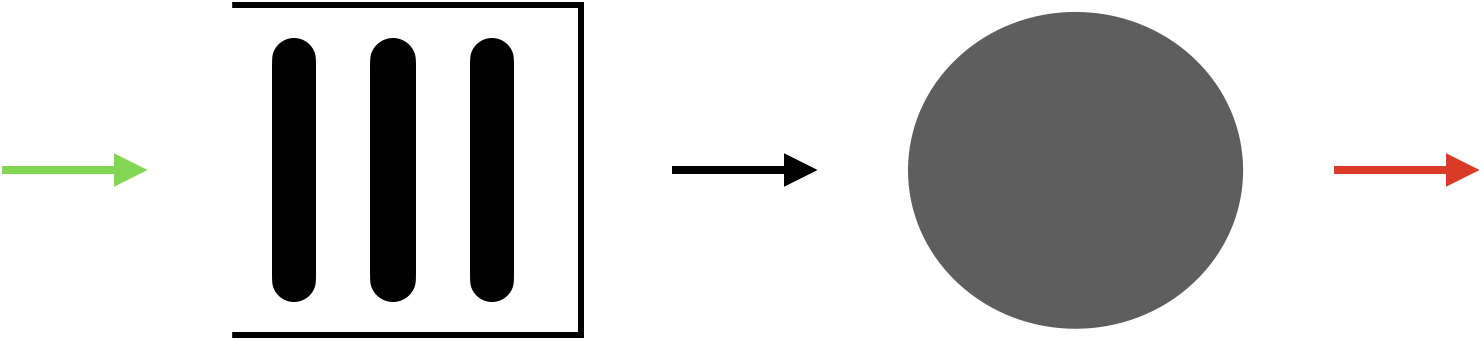
\includegraphics[width=0.3\textwidth]{plot/mm1.png}
  \end{center}
  \caption{$M/M/1$ queue.} \label{fig:MM1}
\end{wrapfigure}

There are two boundary cases that make the update slightly different from \eqref{eq:aux_update}. First, if a new job arrives at an empty queue $j$ (either an external arrival or a transition from a job completion), we also need to update $w_{k+1,j}$ to $W_{k+1,j}$. Second, if a queue $j$ job completion leaves an empty queue behind, we set $w_{k+1, j} = \infty$, indicating that no completions can occur for an empty queue.
%If the queue is emptied, then the workload is $W_{k} = \infty$, indicating that no completions can occur for an empty queue. 



Let $\xi_{k}$ denote exogenous noise in the environment, which consists of the sampled inter-arrival times and workloads for resetting the time of a completed event,
\[
\xi_{k} = (T_{k}, W_{k}) \in \R_{+}^{2n}.
\]
We finally arrive at the stated goal of describing the transition dynamics of $s_{k} = (x_{k}, \aux_{k})$ in terms of a function $f(s_{k}, u_{k}, \xi_{k+1})$. Notably, all the stochasticity is captured by $\xi_k$'s, which are independent of the states and actions. 

%As we will discuss in detail later, this results in a special structure for the multi-class queuing network.
% \begin{align}
% %\text{where }
% T & =\{T_{j}\}_{j=1}^{n} \text{ and } T_{j}  \stackrel{iid}{\sim} F_{j}^{A}, \hspace{1em} \forall j \in 1,...,n \\
% %\text{and } 
% W&  =\{W_{j}\}_{j=1}^{n} \text{ and } W_{j}  \stackrel{iid}{\sim} F_{j}^{S}, \hspace{1em} \forall j \in 1,...,n
% % , \quad
% % W_{j} \stackrel{iid}{\sim} F_{j}^{S},\qquad  
% %\tag{Aux Update}
% \end{align}

% The event with the minimum residual time thus is updated to have a residual event time of zero. A new event time is then redrawn for that event, either from $F_{A_{j},t}$ for an arrival or $F_{S_{j}, t}$ for a service time.
% In particular, the update increases the queue length of queue $j$ by $1$ when the next event is an external class $j$ arrival, and it updates the queue lengths according to $R_{j}$ when the next event is a service completion of a class $j$ job. The time update reduces all the residual event times by the ``realized" event time. The rescaling term $\nu(u_{k})^{-1}$ only affects the service times and it rescales to make sure that the service requirements are properly updated. 


% To describe state transitions, we re-iterate that the queue lengths are updated through one of two types of events: arrivals and departures (service completions). In particular, let $E$ denote the set of events $E$. Then, $E=A\cup S$ with $A=\bigcup_{j=1}^{n}A_{j}$ and $S=\bigcup_{j=1}^{n}S_{j}$,
% where arrivals are represented as $A_{j}=e^{j}$ and departures are represented as
% $S_{j}=e^{n+j}$, and (abusing notation) $e^{j}$ is the one-hot vector with 1 in the $j$th position. \hntodo{What is the logic for using subscripts vs superscripts sometimes? The inconsistency might be confusing for some readers. }
% \hntodo{Explicitly say you abuse notation and overload indicator functions for sets, sets themselves, and basis functions.}

% We index the sequence of events by $k\in\mathbb{N}$. We let $\tau_{k}^{A_{j}}$
% be the residual inter-arrival time for queue $j$ right after the $k$th
% event occurred. Likewise, $\tau_{k}^{S_{j}}$ is the residual
% service requirement for top-of-queue job in queue $j$ immediately
% after the $k$th event, with $\tau_{k}^{S_{j}}/u_{j}^{\top}\mu_{j}$
% as the residual processing time. Let $\tau_{k} = (\tau_{k}^{A_{1}},...,\tau_{k}^{A_{n}},\tau_{k}^{S_{1}}/u_{1}^{\top}\mu_{1},...,\tau_{k}^{S_{n}}/u_{n}^{\top}\mu_{n}) \in \mathbb{R}^{2n}$ be the vector of arrival and departure times right after the $k$th event occurred. The $(k+1)$th inter-event time $\tau^{*}_{k+1}$
% is the minimum of all residual inter-event times, i.e., $\tau^{*}_{k+1}=\min \tau_k$.
% %$\min_{i\in[n]}\{\tau_{k}^{A_{j}},\tau_{k}^{S_{j}}/u_{j}^{\top}\mu_{j}\}$.
% The $(k+1)$the event is either an arrival or a departure
% to one of the queues $j\in[n]$, depending on which event has the
% shortest remaining time, i.e., %More specifically, $\event_{k+1}$ is $e^{j}$

% \[
% \event_{k+1}^*=\mathsf{argmin}(\tau_{k}) = 
% \begin{cases}
%     e^{j} &\text{ if } \tau^{*}_{k+1}=\tau_{k,i}^{A} \\
%     e^{n+j} &\text{ if }\tau^{*}_{k+1}=\tau_{k}^{S_{j}}/u_{j}^{\top}\mu_{j}
% \end{cases}
% \]
% Note that in our notation $\argmin$ outputs a one-hot vector in $\R^{2n}$, rather than the index of the event that achieves the minimum. Altogether:
% \begin{align}
% \event_{k+1}^* & =\mathsf{argmin}(\tau_{k}) = \mathsf{argmin} \left\{
% \tau_{k}^{A_{1}},...,\tau_{k}^{A_{n}},
% \frac{\tau_{k}^{S_{1}}}{u_{1}^{\top}\mu_{1}},...,\frac{\tau_{k}^{S_{n}}}{u_{n}^{\top}\mu_{n}}
% \right\}\tag{Event Selection}
% \\
% \tau^{*}_{k+1} & =\min (\tau_{k}) = 
% \min \left\{
% \tau_{k}^{A_{1}},...,\tau_{k}^{A_{n}},
% \frac{\tau_{k}^{S_{1}}}{u_{1}^{\top}\mu_{1}},...,\frac{\tau_{k}^{S_{n}}}{u_{n}^{\top}\mu_{n}}
% \right\}
% \tag{Inter-event Time}
% \end{align}
% \hntodo{Explicitly write $= \event_{k+1}^{*T} \tau_k$ in the final equality}
% Once the event occurs, we update the residual inter-arrival and service
% requirements: arrivals are decremented by $\tau_{k+1}^*$ and service
% requirements are reduced by the amount of work applied to them, which
% is $(u_{j}^{\top}\mu_{j})\tau_{k+1}^*$. If the residual event time reaches zero, it is re-drawn from the corresponding event-time distribution, i.e., $\tau^{A_{j}} \sim F_{A_{j},t}$ and $\tau_{j}^{S} \sim F_{A_{j},t}$ \hntodo{Same type as above}
% \begin{align}
% \text{\ensuremath{\tau_{k+1,i}^{S_{j}}}} & =\begin{cases}
% \tau_{k}^{S_{j}}-(u_{j}^{\top}\mu_{j})\tau^{*}_{k+1} & \text{if }S_{j}\neq \event_{k+1}^*\\
% \tau^{S_{j}}\sim F_{S_{j},t_{k+1}} & \text{otherwise}
% \end{cases}\tag{Service Time Update}\\
% \tau_{k+1,i}^{A_{j}} & =\begin{cases}
% \tau_{k}^{A_{j}}-\tau^{*}_{k+1} & \text{if }A_{j}\neq \event_{k+1}^*\\
% \tau^{A_{j}}\sim F_{A_{j},t_{k+1}} & \text{otherwise}
% \end{cases}\tag{Arrival Time Update}\\
% t_{k+1} & =t_{k}+\tau^{*}_{k+1}\tag{Time Update}
% \end{align}
% \hntodo{What is $i$ here?}
% The system state variable, i.e. queue-lengths, is updated as a linear function of the event:
% \begin{align}
% \label{eq:state_update}
% x_{k+1}=x_{k}+D \event_{k+1} \tag{State Update}
% \end{align}

% In other words, when the next event is an arrival to queue $j$, i.e.
% $\event_{k+1}^*=A_{j}=e^{j}$, then the update is $x_{k+1}=x_{k}+D \event_{k+1}^*=x_{k}+e^{j}$
% which increases the queue $j$ by $1$. Whereas if
% a departure occurs $\event_{k+1}^*=S_{j}=e^{n+j}$, then the state update
% is $x_{k}+D \event_{k+1}=x_{k}+R_{j}$ which is the state update when
% a job from queue $j$ finishes service.

% In total, the dynamics of the multi-class queuing network
% starting from $(x_{k},\tau_{k}^{E},t_{k})$ is,
% \begin{align*}
% x_{k+1} & =x_{k}+D \event_{k+1}\tag{Linear State Update}\\
% \event_{k+1} & =\mathsf{argmin}\cup_{i=1}^{n}\{\tau_{k}^{A_{j}},\tau_{k}^{S_{j}}/u_{j}^{\top}\mu_{j}\}\tag{Event Selection}\\
% \tau_{k+1} & =\min_{i\in[n]}\{\tau_{k}^{A_{j}},\tau_{k}^{S_{j}}/u_{j}^{\top}\mu_{j}\}\tag{Inter-event Time}\\
% \text{\ensuremath{\tau_{k+1,i}^{S_{j}}}} & =\begin{cases}
% \tau_{k}^{S_{j}}-(u_{j}^{\top}\mu_{j})\tau_{k} & \text{if }S_{j}\neq e_{k}\\
% \tau^{S_{j}}\sim F_{S_{j},t_{k+1}} & \text{otherwise}
% \end{cases}\tag{Service Time Update}\\
% \tau_{k+1,i}^{A_{j}} & =\begin{cases}
% \tau_{k}^{A_{j}}-\tau_{k} & \text{if }A_{j}\neq e_{k}\\
% \tau^{A_{j}}\sim F_{A_{j},t_{k+1}} & \text{otherwise}
% \end{cases}\tag{Arrival Time Update}\\
% t_{k+1} & =t_{k}+\tau_{k+1}\tag{Time Update}
% \end{align*}

% \hntodo{This might be better as a figure and putting in the middle of this subsection}
It is worth mentioning a few features of this discrete-event representation.
\begin{itemize}[itemsep=0pt]
    \item While auxiliary data $\aux_{k} = (\tau^{A}_{k}, w_{k})$ is necessary for $s_{k} = (x_{k}, \aux_{k})$ to be a valid Markovian system descriptor, this information is typically not available to the controller. We assume the controller only observes the queue lengths, i.e., the control policy $\pi$ only depends on $x_k$.
    \item The representation can flexibly accommodate non-stationary and non-exponential event-time distributions, i.e., $F_{j}^{A}$'s and $F_{j}^{S}$'s can be general and time-varying.
    \item This model enables purely data-driven simulation, as it only requires samples of the event times $\xi_{k}$. One does not need to know the event time distributions $F_{j}^{A}$'s and $F_{j}^{S}$'s to simulate the system if data of these event times are available.
    \item The matrix-vector representation enables GPU parallelism, which can greatly speed up the simulation of large-scale networks. 
    %It also enables efficient evaluation of several trajectories in parallel.
    \item As we will explain later, this representation enables new gradient estimation strategies.
\end{itemize}


\paragraph{Queuing Network Examples}
As a concrete illustration, we show how a few well-known queuing networks are described as discrete-event dynamical systems.
% \hntodo{Split the figure and put it in each example via wrapfigure}
\vspace{1em}



\begin{example}
\label{example:mm1}
The $M/M/1$ queue (see Figure \ref{fig:MM1}) with arrival rate $\lambda>0$ and
service rate $\mu\geq\lambda$ features a single queue $n=1$ and a single server $m=1$, and exponentially distributed inter-arrival times and workloads, i.e., $T_k \sim \mathsf{Exp}\left(\lambda\right)$ and
$W_k \sim \mathsf{Exp}(1)$ respectively. The network topology is $M=[1]$, the service rate is $\mu$, and the routing matrix is $R =[-1]$, indicating that jobs leave the system after service completion.
The scheduling policy is work-conserving, the server always serves the queue when it is non-empty, i.e. $u_{k}=1\{x_{k}>0\}$. The state update is,
\begin{align*}
 x_{k+1}  &=x_{k}+\left[\begin{array}{cc}
1 & -1
\end{array}\right]^{\top}\event_{k+1}\\
\event_{k+1} 
&=\arg\min\left\{ \tau_{k}^{A},\tau_{k}^{S} \right\} =\arg\min\left\{ \tau_{k}^{A},\frac{\servicek}{\mu \cdot 1\{x_{k}>0 \}} \right\} \in \{0,1\}^{2} \\
\tau^{*}_{k+1} &= \min\left\{ \tau_{k}^{A},\tau_{k}^{S} \right\} \\
\left[
\begin{array}{c}
\tau_{k+1}^{A} \\
w_{k+1}
\end{array}
\right]
&= 
\left[
\begin{array}{c}
\tau_{k}^{A} \\
w_{k}
\end{array}
\right]
- \tau_{k+1}^{*}\left[
\begin{array}{c}
1 \\
\mu 1\{ x_{k} > 0\}
\end{array}
\right] +
\left[
\begin{array}{c}
T_{k+1} \\
W_{k+1}
\end{array}
\right] \odot e_{k+1}.
\end{align*}
%The event matrix is  $D=[1,-1]$, indicating that the queue increases by 1 when an arrival occurs and decreases by 1 when a job completion occurs. 
%Note that since $(T_{k}, W_{k})$ are independent exponential random variables, $(\tau_{k}^{A}, w_{k})$ are as well for all $k$.
\end{example}



\begin{example}
\label{example:multiclass}
The {\bf multi-class singer-server queue} features an $n$ queues and a single server $m=1$ (see Figure \ref{fig:multi-class}). While the inter-arrival times and workloads, i.e., $(T_{k}, W_{k})$'s are usually exponentially distributed, they can also follow other distributions. The network topology is $M=[1,...,1] \in \R^{n}$, the service rates are $\mu = [\mu_{1},...,\mu_{n}]$, and the routing matrix is $R =[-1,...,-1]\in \R^{n}$, indicating that jobs leave the system after service completion. 
A well-known scheduling policy for this system is the $c\mu$-rule, a static priority rule.
%based on the holding costs and service rate and is known to be optimal for this network. 
Let $h = (h_{1},...,h_{n}) \in \R^{n}$ denote the holding costs. The $c\mu$-rule sets
\[
    u_{k}=\argmax_{j\in [n]} \{ h_{j}\mu_{j}1\{x_{j}>0\} \}\in \{0,1\}^{n}.
\]
%where $\argmax$ maps a vector into a one-hot vector indicating the index of the arg max. 
The state update is,
\begin{align*}
 x_{k+1}  &=x_{k}+\left[\begin{array}{cc}
\ones_{n} & -\ones_{n}
\end{array}\right]^{\top}\event_{k+1}\\
\event_{k+1} 
&=\arg\min\left\{ \tau_{k,1}^{A},...,\tau_{k,n}^{A},\tau_{k,1}^{S},...,\tau_{k,n}^{S} \right\} 
=\arg\min\left\{ \tau_{k,1}^{A},...,\tau_{k,n}^{A},
\frac{w_{k,1}}{\mu_{1} u_{k,1}},...
\frac{w_{k,n}}{\mu_{n} u_{k,n}}\right\} \\
\tau^{*}_{k+1} &= \min\left\{ \tau_{k,1}^{A},...,\tau_{k,n}^{A},\tau_{k,1}^{S},...,\tau_{k,n}^{S} \right\} \\
\left[
\begin{array}{c}
\tau_{k+1}^{A} \\
w_{k+1}
\end{array}
\right]
&= 
\left[
\begin{array}{c}
\tau_{k}^{A} \\
w_{k}
\end{array}
\right]
- \tau_{k+1}^{*}\left[
\begin{array}{c}
\ones_{n} \\
\mu \odot u_{k}
\end{array}
\right] +
\left[
\begin{array}{c}
T_{k+1} \\
W_{k+1}
\end{array}
\right] \odot e_{k+1}.
\end{align*}
%where $\odot$ is element-wise multiplication. 
\end{example}


\begin{example}
\label{example:criss-cross}
The {\bf criss-cross network}~\cite{harrison1990scheduling} features $n=3$ queues and $m=2$ servers (see Figure~\ref{fig:networks}). External jobs arrive to queues 1 and 3. The first server can serve queues 1 and 3 with service rates $\mu_{11}$ and $\mu_{13}$ respectively, while the second server is dedicated to serving queue 2 with service rate $\mu_{22}$. After jobs from queue 1 are processed, they are routed to queue 2; jobs from queues 2 and 3 exit the system after service completion. The inter-arrival times and workloads, i.e., $(T_{k}, W_{k})$'s, can follow general distributions.
The network topology $M$, service rate matrix, and the routing matrix $R$ are:
\[
M = \left[ \begin{array}{ccc}
1 & 0 & 1\\
0 & 1 & 0 \\
\end{array} \right], \qquad
\mu = \left[ \begin{array}{ccc}
\mu_{11} & 0 & \mu_{13}\\
0 & \mu_{22} & 0 \\
\end{array} \right], \qquad
R = \left[ \begin{array}{ccc}
-1 & 0 & 0\\
1 & -1 & 0 \\
0 & 0 & -1
\end{array} \right]
\]
%At every step $k$, the action $u_{k}\in \{0,1\}^{m \times n}$ is constrained so that $u_{k,11} + u_{k,13}\leq 1$, $u_{k,22}\leq 1$. 
\citet{harrison1990scheduling} develop a work-conserving threshold policy for this system. For a threshold $a \in \N_{+}$, server 1 prioritizes jobs in queue 1 if the number of jobs in queue 2 is below $a$. Otherwise, it prioritizes queue 3. This gives the scheduling action
\[
u_{k,11} = 1\{x_{k,2} \leq a \}, \quad
u_{k,22} = 1\{x_{k,2} > 0 \}, \quad 
u_{k,13} = (1 - u_{k,11})1\{x_{k,3} > 0\},
\]
and the transition dynamics 
\begin{align*}
 x_{k+1}  &=x_{k}+\left[\begin{array}{cc}
I_{3} & R
\end{array}\right]
\event_{k+1}\\
\event_{k+1} &=\arg\min\left\{ 
\tau_{k,1}^{A}, \infty, \tau_{k,3}^{A}, 
\tau_{k,1}^{S},
\tau_{k,2}^{S},
\tau_{k,3}^{S}
\right\}  
=\arg\min\left\{ 
\tau_{k,1}^{A}, \infty, \tau_{k,3}^{A}, 
\frac{w_{k,1}}{\mu_{11}u_{k,11}},
\frac{w_{k,2}}{\mu_{22}u_{k,22}}, 
\frac{w_{k,3}}{\mu_{13}u_{k,13}}\right\}  \\
\tau^{*}_{k+1} &= \min\left\{ 
\tau_{k,1}^{A}, \infty, \tau_{k,3}^{A}, 
\tau_{k,1}^{S},
\tau_{k,2}^{S},
\tau_{k,3}^{S}\right\} \\
\left[
\begin{array}{c}
\tau_{k+1}^{A} \\
w_{k+1}
\end{array}
\right]
&= 
\left[
\begin{array}{c}
\tau_{k}^{A} \\
w_{k}
\end{array}
\right]
- \tau_{k+1}^{*}\left[
\begin{array}{c}
\ones_{3} \\
\servicemapk
\end{array}
\right] +
\left[
\begin{array}{c}
T_{k+1} \\
W_{k+1}
\end{array}
\right] \odot e_{k+1}.
\end{align*}
Here, $\tau_{k,2}^{A} = \infty$ since queue 2 has no external arrivals. 
%While usually $(T_{k}, W_{k})$ are independent exponential random variables, this need not be the case.
%Only jobs from queue 1 that have finished processing are routed to queue 2.
% Jobs leave the system after processing so $R=-1$, and the event matrix is  $D=[1,-1]$. 
\end{example}






% \begin{remark}
% (Pre-emptive service) In this work, we focus on \textbf{pre-emptive}
% service disciplines, which allow servers to be routed to another job
% without having to complete their current job. In such cases, the service
% to the interrupted job is paused and can be restarted if the server
% is routed back to the job. 
% %This means that interrupted work is preserved and pre-emptive service policies can route jobs freely without violating work-conservation.
% \end{remark}


% \begin{remark}
% (Buffer sizes) If the queuing network has fixed buffer-sizes $B=\{B_{j}\}_{j=1}^{n}\in\mathbb{N}_{+}^{n}$,
% which prevents jobs from joining queue $j$ if it exceeds the buffer
% $B_{j}$, then the state update is modified as follows
% \[
% x_{k+1}=\min\{x_{k}+D \event_{k+1},B\}\tag{Buffer State Update}
% \]
% The buffer $B$ can be chosen by the controller, or even can be adjusted dynamically. \end{remark}
%

% \subsection{The Multiclass Queuing Network is an Exogenous MDP}
% \label{subsec:exo-mdp}

% An important observation from the above system description is that the dynamics of the multi-class queuing network are ``almost" deterministic: all the randomness is in the inter-arrival times and service requirements drawn from the environment whenever an arrival or service completion occurs. As a result, it is an Exogenous Markov Decision Process (Exo-MDP) ~\cite{sinclair2023hindsight, madeka2022deep}, which is a special class of MDPs in which randomness in the state transitions can be attributed to exogenous random variables $\xi_k$'s. 

% Recall that the state of the discrete event system involves queue lengths and auxiliary state information, i.e., $s_{k}=(x_{k},\aux_{k})$.
% As mentioned earlier, the state transition of $s_{k}$ can be written as,
% \[
% s_{k+1}=f(s_{k},u_{k},\xi_{k}).
% \]
% %where $f$ is the transition function described above and $\xi_{k}=(T_{k}, W_{k}) \in\mathbb{R}^{2n}$ are sampled iid inter-arrival times and workloads sampled.
% Exogeneity relies on two facts:
% \begin{enumerate}
% \item The distributions $F_{j}^{S}$ and $F_{j}^{A}$ do not depend on the
% state $s_{k}$ or action $u_{k}$.
% \item The exogenous state $\xi_{k}$ includes {\color{blue} independently} drawn arrival times and service requirements for \emph{all} queues, not only for the queue which experiences an arrival or service completion.
% \end{enumerate}
% This exogenous structure allows one to simulate trajectories of the
% system from different states and under counterfactual actions using
% just a single trace $\xi_{1:N}$ of stochastic inputs. As a result,
% this enables offline learning from a dataset of traces. 
% Note that
% although reinforcement learning in Exogenous MDPs have been studied in recent years, this exogenous structure has been observed since the 1990s (cite Christos
% paper).




%%% Local Variables:
%%% mode: latex
%%% TeX-master: "main"
%%% End:
